\documentclass[a4paper]{amsart}

%                  XeTeX
%\usepackage{xunicode}
%\usepackage{fontspec}
%\usepackage{xltxtra}
%setromanfont[Mapping=tex-text]{Linux Libertine O}

%                  Trash .aux file after toggling
\usepackage{stmaryrd}
\usepackage{graphicx}
\usepackage[margin=1in]{geometry}
\usepackage[lutzsyntax]{virginialake}\aftrianglefalse
\usepackage[pdfborder={0 0 0}]{hyperref}

%--------- Theorem etc
\newtheorem{thm}{Theorem}[section]
\newtheorem{cor}[thm]{Corollary}
\newtheorem{lem}[thm]{Lemma}
\newtheorem{pro}[thm]{Proposition}

\theoremstyle{remark}
\newtheorem{rem}[thm]{Remark}

\theoremstyle{definition}
\newtheorem{defi}[thm]{Definition}
%---------

%-------------------------------------------------------- REMOVE WHEN PAPER DONE
\newcommand{\Ale}[1]{{\color{red}\noindent {\bf A:} #1}}
\newcommand{\Tom}[1]{{\color{green}\noindent {\bf T:} #1}}
\newcount\todocount\todocount=0
\newcommand{\TODO}[1]{\global\advance\todocount by1%
            {\color{red}\noindent{\bf\the\todocount\ TODO:} #1}}\vlupdate{\TODO}
\renewcommand{\Ale}[1]{\relax}  % Comment/uncomment these three lines
\renewcommand{\Tom}[1]{\relax}  % in order to display/hide inline comments
%\renewcommand{\TODO}[1]{\relax} %
%-------------------------------------------------------- REMOVE WHEN PAPER DONE

\begin{document}

\title[Normalisation Control in Deep Inference   via Atomic Flows II]
      {Normalisation Control in Deep Inference\\ via Atomic Flows II}

\author{Alessio Guglielmi and Tom Gundersen}
%\address{University of Bath, Bath BA2 7AY, UK}

\thanks{This work was in part funded by an Overseas Research Scholarship and a Research Studentship, both from the University of Bath, and by the British Council Alliance Programme.}

\keywords{Normalisation, deep inference, cut elimination, atomic flows}

\subjclass{F.4.1 Mathematical Logic---Proof theory}

% \begin{abstract}
% \end{abstract}

\maketitle

%===============================================================================
% \section{Introduction}
\newcommand{\ot}{\mathbin\shortleftarrow}
\newcommand{\fff}{\mathsf f}
\newcommand{\ttt}{\mathsf t}
\newcommand{\ai}{\mathsf{ai}}
\newcommand{\aw}{\mathsf{aw}}
\newcommand{\ac}{\mathsf{ac}}
\newcommand{\aid}{{\ai{\downarrow}}}
\newcommand{\awd}{{\aw{\downarrow}}}
\newcommand{\acd}{{\ac{\downarrow}}}
\newcommand{\aiu}{{\ai{\uparrow}}}
\newcommand{\awu}{{\aw{\uparrow}}}
\newcommand{\acu}{{\ac{\uparrow}}}
\newcommand{\swi}{\mathsf{s}}
\newcommand{\med}{\mathsf{m}}
\newcommand{\sus}{\mathsf{ss}}
\newcommand{\said}{\mathsf{s}\aid}
\newcommand{\contr}{\mathsf{c}}
\newcommand{\cod}{{\contr{\downarrow}}}
\newcommand{\cou}{{\contr{\uparrow}}}
\newcommand{\SKS}{\mathsf{SKS}}
\newcommand{\ppl  }{{\mathchoice{\scriptstyle+}
                                {\scriptstyle+}
                                {\scriptstyle+}
                                {\scriptscriptstyle+}}}
\newcommand{\pmi  }{{\mathchoice{\scriptstyle-}
                                {\scriptstyle-}
                                {\scriptstyle-}
                                {\scriptscriptstyle-}}}

% \Ale{were the previous methods crap?}
%
% \Tom{in my opinion the method shown here is a strict improvement, let me know if you know of any downsides (I might have forgotten)}
%
% \Ale{global?}
%
% In \cite{GuglGund:07:Normalis:lr} we introduced \emph{atomic flows} as a tool to study normalisation. In this paper we focus on global normalisation procedures and show how they provide for more general and principled tools than what we studied before. The paper is in two parts, the first part gives a \emph{confluent} cut-elimination procedure for propositional classical logic and the second part gives a generalisation of the \emph{streamlining} procedure described in \cite{GuglGund:07:Normalis:lr}.
%
% \Ale{is the causual relationship known?}
%
% Atomic flows are graphical representations of derivations conserving their size as well as the causal relationship between the structural inference rules. All information about logical connectives and logical inference rules is disregarded. The crucial property of atomic flows is that they contain all the information necessary to perform normalisation. We can either just normalise the atomic flows, or use the atomic flows to decide how to normalise the derivations.
%
% \Ale{previous sentence, see hand written comments [could not read comment]}
%
% A streamlined derivation is a derivation whose atomic flow has a specific shape, in particular this entails that
%
% \begin{enumerate}
% \item a streamlined derivation contains no causal relationship between an axiom and a cut; and
% \item in the special case where the premiss of a streamlined derivation is $\ttt$, the derivation is cut-free.
% \end{enumerate}
%
% \Ale{causal relationship not understandable}
%
% \Ale{put a picture}
%
% \Tom{will do (later, when the text is finished)}
%
% Given the atomic flow of a derivation, we can tell what the atomic flow of the streamlined derivation would be. This is of particular interest because the atomic flows do not have access to any information about logical inference rules. This is remarkable because the relationship of the logical inference rules is usually considered crusial to have cut-elimination.
%
% The novelty of this work is to only use global proof transformations when performing normalisation. We single out axioms and cuts and consider the rest of the atomic flow to be inside `black boxes' which we do not need to look inside. Then, by knowing which axioms are connected with which cuts, we can normalise the derivation without having any more information about its internal structure. The streamlining procedures presented in \cite{GuglGund:07:Normalis:lr} had two sources of exponential growth, it was not strongly normalising and the proof of termination was not very intuitive. With the new methods we have removed one source of exponential growth and both termination and strong normalisation are immediate.
%
% \Ale{was there anything good about the previous paper?}
% \Ale{isn't strong normalisation enough?}
%
% \section{Deep Inference and Atomic Flows}
%
% Deep inference is a relatively new proof-theoretic methodology developed over the past ten years. Deep inference differs from the traditional Gentzen-style methodology in that it allows inference at any level in formulae, not only at the root connective. This allows for much greater freedom in designing formalisms and logical systems, but it also makes normalisation theory much more challenging.
%
% In this paper, we are working in the deep-inference formalism `calculus of structures' \cite{Gugl:06:A-System:kl}, but the results here are not specific to this formalism as we will discuss later.
%
% The system we use for propositional classical logic is system $\SKS$ \cite{BrunTiu:01:A-Local-:mz}:
%
% \Ale{adjust spacing}
%
% \begin{figure}[h]
% \begin{center}
% \begin{tabular}{ccc}
% $\vlinf{\aid}{}{\vls[a.\bar{a}]}{\ttt}$ & $\vlinf{\acd}{}{a}{\vls[a.a]}$ & $\vlinf{\awd}{}{a}{\fff}$ \\
% interaction (axiom) & contraction & weakening \\
% \noalign{\bigskip}
% \\
% $\vlinf{\aiu}{}{\fff}{\vls(\bar{a}.a)}$ & $\vlinf{\acu}{}{\vls(a.a)}{a}$ & $\vlinf{\awd}{}{\ttt}{a}$ \\
% cointeraction (cut) & cocontraction & coweakening \\
% \noalign{\bigskip}
% \\
% \end{tabular}
% \begin{tabular}{cc}
% $\vlinf{\swi}{}{\vls[(\alpha.\beta).\gamma]}{\vls(\alpha.[\beta.\gamma])}$ &
% $\vlinf{\med}{}{\vls([\alpha.\beta].[\gamma.\delta])}{\vls[(\alpha.\gamma).(\beta.\delta)]}$ \\
% switch & medial
% \end{tabular}
% \end{center}
% \end{figure}
%
% Furmulae are considered equal modulo associativity and commutativity of $\wedge$ and $\vee$, and idempotency and identity of $\ttt$ and $\fff$. Furthermore, negation is only allowed on atoms which is possible due to De Morgan's laws.
%
% In this paper we will mainly concern ourselves with the structural rules.
%===============================================================================
\section{Streamlining via Experiments}

\begin{lem}\label{LemSuperSwitch}
Given a context $\xi\vlhole$ and a formula $\alpha$ there exist derivations $\vlder{}{\{\swi\}}{\xi\{\alpha\}}{\vls(\alpha.\xi\{\ttt\})}$ and $\vlder{}{\{\swi\}}{\vls[\xi\{\fff\}.\alpha]}{\xi\{\alpha\}}$.
\end{lem}

\begin{proof}
We show how to construct the first derivation, the second one can be done by symmetry. We argue by induction on the number of atoms in $\xi\vlhole$. There are three cases to consider, where $\beta$ is not a unit:
\begin{itemize}
  \item $\xi\vlhole=\vlhole$,
  \item $\xi\vlhole=\vls[\xi'\vlhole.\beta]$,
  \item $\xi\vlhole=\vls(\xi'\vlhole.\beta)$.
\end{itemize}

For each case we can build the required derivation:

\[
\vlinf{=}{}{\alpha}{\vls(\alpha.\ttt)}\quad,\qquad
\vlderivation
{
 \vlin{\swi}{}{\vls[\vlder{\Psi}{\{\swi\}}{\xi'\{\alpha\}}{\vls(\alpha.\xi'\{\ttt\})}.\beta]}
 {
  \vlhy{\vls(\alpha.[\xi'\{\ttt\}.\beta])}
 }
}\qquad\mbox{and}\qquad
\vlderivation
{
 \vlin{=}{}{\vls(\vlder{\Psi'}{\{\swi\}}{\xi'\{\alpha\}}{\vls(\alpha.\xi'\{\ttt\})}.\beta)}
 {
  \vlhy{\vls(\alpha.(\xi'\{\ttt\}.\beta))}
 }
}\quad,
\]
where $\Psi$ and $\Psi'$ exists by the inductive hypothesis.
\end{proof}

\begin{lem}\label{LemContr}
Given a formula $\alpha$ and a positive integer $n$, there exist derivations $\vlder{}{\{\acd,\med\}}{\alpha}{\bigvee_{i=1}^{n}\alpha}$\\ and $\vlder{}{\{\acu,\med\}}{\bigwedge_{i=1}^{n}\alpha}{\alpha}$.
\end{lem}


\begin{defi}
Given a derivation $\Phi$ from $\alpha$ to $\beta$, where $a_1,\dots,a_n$ are all the distinct atoms that appear in both interaction and cointeraction instances, a \emph{core of\ $\Phi$} is defined as a derivation 
\[
\vlder{}{}{\vls[\beta.(a_n.\bar a_n).\cdots.(a_1.\bar a_1)]}{\vls([a_1.\bar a_1].\cdots.[a_n.\bar a_n].\alpha)}
\]
where the atoms $a_1,\dots,a_n$ do not occur in any interaction nor cointeraction instances.
\end{defi}

\begin{lem}\label{LemConstrCore}
Given a derivation $\Phi$ from $\alpha$ to $\beta$, a core of $\Phi$ can be constructed.
\end{lem}

\begin{proof}
Let $a_1,\dots,a_n$ be all the atoms which occur in both interaction and cointeraction instances in $\Phi$. Obtain $\Phi'$ from $\Phi$ by using Lemma~\ref{LemSuperSwitch} to perform the following transformation for each instance of $\aid$ and $\aiu$ applied to $a$ from $a_1,\dots,a_n$ in $\Phi$:
\[
\vlderivation
{
 \vlde{\Psi'}{}{\beta}
 {
  \vlin{\aid}{}{\xi\vlsbr[a.{\bar a}]}
  {
   \vlde{\Psi}{}{\xi\{\ttt\}}
   {
    \vlhy{\alpha}
   }
  }
 }
}\quad\rightarrow\quad
\vlderivation
{
 \vlde{\Psi'}{}{\beta}
 {
  \vlde{}{\{\swi\}}{\xi\vlsbr[a.{\bar a}]}
  {
   \vlhy{\vlsbr([a.{\bar a}].\vlder{\Psi}{}{\xi\{\ttt\}}{\alpha})}
  }
 }
}\qquad\mbox{and}\qquad
\vlderivation
{
 \vlde{\Psi'}{}{\beta}
 {
  \vlin{\aid}{}{\xi\{\fff\}}
  {
   \vlde{\Psi}{}{\xi\vlsbr(a.{\bar a})}
   {
    \vlhy{\alpha}
   }
  }
 }
}\quad\rightarrow\quad
\vlderivation
{
 \vlde{}{\{\swi\}}{\vlsbr[\vlder{\Psi'}{}{\beta}{\xi\{\fff\}}.(a.{\bar a})]}
 {
  \vlde{\Psi}{}{\xi\vlsbr(a.{\bar a})}
  {
   \vlhy{\alpha}
  }
 }
}\quad.
\]

Obtain the core of $\Phi$ from $\Phi'$ by using Lemma~\ref{LemContr}:
\[
\vlderivation
{
 \vlde{}{\{\acd,\med\}}{\vls[\beta.(a_n.{\bar a_n}).\cdots.(a_1.{\bar a_1})]}
 {
  \vlde{\Phi'}{}{\vls[\beta.(a_n.\bar a_n).\cdots.(a_n.\bar a_n).\cdots.(a_1.\bar a_1).\cdots.(a_1.\bar a_1)]}
  {
   \vlde{}{\{\acu,\med\}}{\vls([a_1.\bar a_1].\cdots.[a_1.\bar a_1].\cdots.[a_n.\bar a_n].\cdots.[a_n.\bar a_n].\alpha)}
   {
    \vlhy{\vls([a_1.{\bar a_1}].\cdots.[a_n.{\bar a_n}].\alpha)}
   }
  }
 }
}\quad.
\]
\end{proof}

\begin{defi}
A core of a derivation $\Phi$ constructed as described in the proof of Lemma~\ref{LemConstrCore} is called \emph{the canonical core of $\Phi$}.
\end{defi}

\begin{defi}
For any natural number $n$ the \emph{$n$-normaliser}, $\Psi_n(\Phi,\alpha,\beta,a_1,\dots,a_n)$, is a derivation scheme over the meta variables $\Phi$ (derivation), $\alpha$, $\beta$ (formulae) and $a_1,\dots,a_n$ (atoms), where
\[
\Phi=\vlder{}{}{\vls[\beta.(a_n.{\bar a_n}).\cdots.(a_1.{\bar a_1})]}{\vls([a_1.{\bar a_1}].\cdots.[a_n.{\bar a_n}].\alpha)}\quad.
\]
If $\Phi,\alpha,\beta,a_1,\dots,a_n$ are clear from the context then we use the following shorthand
\[
\Psi_k=\Psi_k(\Phi,\vls([a_{k+1}.\bar a_{k+1}].\cdots.[a_n.\bar a_n].\alpha),\vls[\beta.(a_n.\bar a_n).\cdots.(a_{k+1}.\bar a_{k+1})],a_1,\dots,a_k)\quad.
\]
We define $\Psi_n$ inductively. Let $\Psi_0=\Phi$ and for $n>0$ let $\Psi_n$ be
\newbox\DeltaTopK
\setbox\DeltaTopK=
\hbox{$
\vlderivation
{
 \vlde{\Psi_{n-1}}{}{\vls[\beta.(\vlinf{\awu}{}{\ttt}{a_n}.\bar a_n)]}
 {
  \vlhy{\vls(\vlinf{\aid}{}{\vls[a_n.\bar a_n]}{\ttt}.\alpha)}
 }
}$
}
\newbox\DeltaBotK
\setbox\DeltaBotK=
\hbox{
$\vlderivation
{
 \vlde{\Psi_{n-1}}{}{\vls[\beta.\vlinf{\aiu}{}{\fff}{\vls(a_n.\bar a_n)}]}
 {
  \vlhy{\vls([a_n.\vlinf{\awd}{}{\bar a_n}{\fff}].\alpha)}
 }
}$
}
\newbox\DeltaK
\setbox\DeltaK=
\hbox{$
\vlderivation
{
 \vlde{\Psi_{n-1}}{}{\vls[\beta.(a_n.\vlinf{\awu}{}{\ttt}{\bar a_n})]}
 {
  \vlhy{\vls([\vlinf{\awd}{}{a_n}{\fff}.\bar a_n].\alpha)}
 }
}$
}
\[
\vlderivation
{
 \vlin{\cod^\star}{}{\beta}
 {
  \vlin{\swi}{}{\vls[\beta.\beta.\box\DeltaBotK]}
  {
   \vlin{\swi}{}{\vls([\beta.\box\DeltaK].\alpha)}
   {
    \vlin{\cou^\star}{}{\vls(\box\DeltaTopK.\alpha.\alpha)}
    {
     \vlhy{\alpha}
    }
   }
  }
 }
}\quad.
\]
\end{defi}

\begin{defi}
Given a derivation $\Phi$ from $\alpha$ to $\beta$, where $a_1,\dots,a_n$ are all the atoms that appear in both interaction and cointeraction instances, the \emph{normaliser of $\Phi$} is the derivation obtained by instantiating the $n$-normaliser with the core, premiss and conclusion of $\Phi$ and the atoms $a_1,\dots,a_n$.
\end{defi}

\begin{thm}
The normaliser of any derivation is streamlined.
\end{thm}
\begin{proof}

Consider the atomic flow of the atom $a_k$ in the derivation $\Psi_k$. Note that the interaction and cointeraction evidenced in this atomic flow are the only ones that apply to the atom $a_k$ in $\Psi$. It is straightforward to see that the given atomic flow does not contain any path from the interaction to the cointeraction. This holds for every $a_k$ so $\Psi$ is streamlined.

\begin{center}
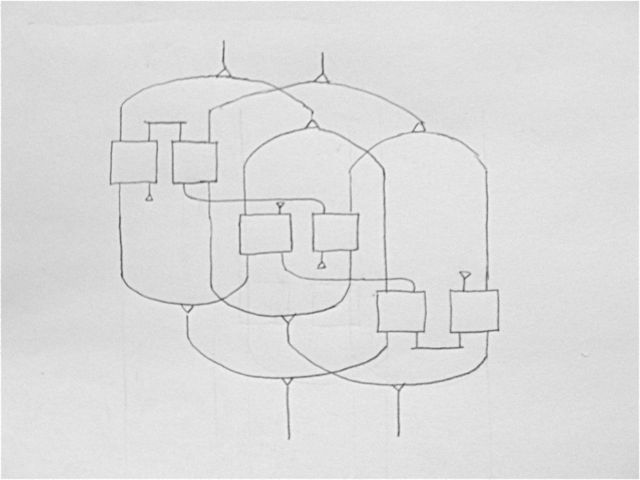
\includegraphics[scale=0.5]{./threeboxes.png}
\end{center}

\end{proof}



% \iflmcs\else\let\oldurl\url\renewcommand{\url}[1]{\hfill\break\oldurl{#1}}\fi
%
% \bibliographystyle{alpha}
% \bibliography{di-biblio}

\end{document}